---
title: Congruences and Quotient Algebras
summary: On equating equivalent objects.
header-img: /images/congruences.png
header-img-alt: An illustration of a quotient algebra hatching from an egg
tags: math, universal algebra
---

\documentclass{article}
\usepackage{amsmath}
\begin{document}
Previously: \href{/posts/2021-04-02-algebras.html}{Algebras}

Suppose we have an algebra $(X, F)$ where $X$ is a set of elements and $F$ is a set of operations. We would like to construct a smaller algebra from $(X, F)$ that still "preserves the operations in $F$" in some sense.

Why would anyone do this? Think of this smaller algebra as the original algebra with some information abstracted away. In my previous post, I demonstrated how you can use certain algebras to model the integers under addition or logical propositions. You may want to examine relationships not between individual elements, but collections of elements that behave similarly under the algebra's operations, like the relationship between even and odd integers, or logical propositions that become logically equivalent if some statement is assumed to be true. If you collapse each collection of similar elements to a single element in the new algebra, you can ignore intra-collection differences and focus on inter-collection differences. 

A reasonable starting point is to consider the image of $(X, F)$ under a homomorphism. Homomorphisms are functions between the element sets of algebras of the same type that preserve operations: for any $m: (X, F) \to (X', F)$ and any $f$ in $F$, $m(f(x_0, x_1 \dots x_n)) = f(m(x_0), m(x_1) \dots m(x_n))$ (since $(X, F)$ and $(X', F)$ are of the same type, $f$ is an operation on both $X$ and $X'$). $m$ can map two elements of $X$ to the same output, but can never map one element to more than one distinct output. So the image of $(X, F)$ under $m$ looks like $(X, F)$ with 0 or more its points identified. Let's describe the image in terms of a relation on $(X, F)$: $R(x, y)$ if and only if $m(x) = m(y)$.

\begin{figure}
\includegraphics{/images/export-6-1.webp}
\caption{The image of a finite lattice under a homomorphism.}
\end{figure}

\begin{figure}
\includegraphics{/images/export-7.webp}
\caption{The image of the group $(\mathbb{Z}, +, 0, 1)$ under a homomorphism.}
\end{figure}

Can we identify any points we want, i. e, can we find a homomorphism m whose image corresponds to any arbitrary relation $R$? Not if we want equality to make sense:

\begin{itemize}
\item{if R isn't reflexive, then $\neg R(x, x)$ implies $m(x) \neq m(x)$}
\item{if R isn't symmetric, then $R(x, y) $ and $\neg R(y, x)$ implies $m(x) = m(y)$, but $m(y) \neq m(x)$}
\item{if R isn't transitive, then $R(x, y), R(y, z)$ and $\neg R(x, z)$ implies $m(x) = m(y)$ and $m(y) = m(x)$, but $m(x) \neq m(z)$}
\end{itemize}

So $R$ has to be an \href{https://mathworld.wolfram.com/EquivalenceRelation.html}{equivalence relation}. Moreover:

if $R(x_0, y_0), R(x_1, y_1) \dots R(x_n, y_n)$ 

 and

$\neg R(f(x_0, x_1 \dots x_n), f(y_0, y_1, \dots y_n))$, then 

$m(f(x_0, x_1 \dots x_n)) \neq m(f(y_0, y_1 \dots y_n))$

which contradicts the fact that the homomorphism $m$ preserves operations, since

$m(x_0) = m(y_0) , \dots, m(x_n) = m(y_n)$ 

implies that 

$f(m(x_1 ),\dots, m(x_n)) = f(m(y_1), \dots, m(y_n)) = m(f(x_1, x_2, \dots,  x_n)) = m(f(y_1, y_2, \dots, y_n))$

So $R$ must also "preserve operations".

\begin{figure}
\includegraphics[options]{/images/export-8.webp}
\caption{Any relation on this finite lattice $(\{a, b, c, d, e\}, \land, \lor\)$ such that $R(c, e)$ but not $R(c, d)$ and $R(d, e)$ is not a congruence relation.}
\end{figure}

\begin{figure}
\includegraphics[options]{/images/export-9.webp}
\caption{Any relation on the group $(\mathbb{Z}, +, 0, -)$ such that $R(-1, 1)$ but $\neg R(-n, n)$ for some $n \in \mathbb{Z}$ is not a congruence relation.}
\end{figure}

This gives us the \textbf{definition of a congruence: an equivalence relation on the elements of an algebra that preserves operations.} Given a congruence $R$ on an algebra $(X, R)$, \textbf{we form the quotient algebra $(X, F)/R$ where the set of elements is the set of equivalence classes of $R$, and the operations are the operations of $F$ applied to equivalence classes}. The equivalence class $[b]_R$ is the set of all elements $x \in X$ such that $R(b, x)$. The operations of $F$ are well-defined on equivalence classes of $R$ because $R$ preserves operations: if $R(x_0, y_0) \dots R(x_n, y_n)$ and $f(x_0 \dots x_n) = x$, $f(y_0 \dots y_n) = y$, then $R(x, y)$, so:

$f([x_0]_R \dots [x_n]_R) = f([y_0]_R \dots [y_n]_R)  = [x]_R = [y]_R.$
\begin{figure}
    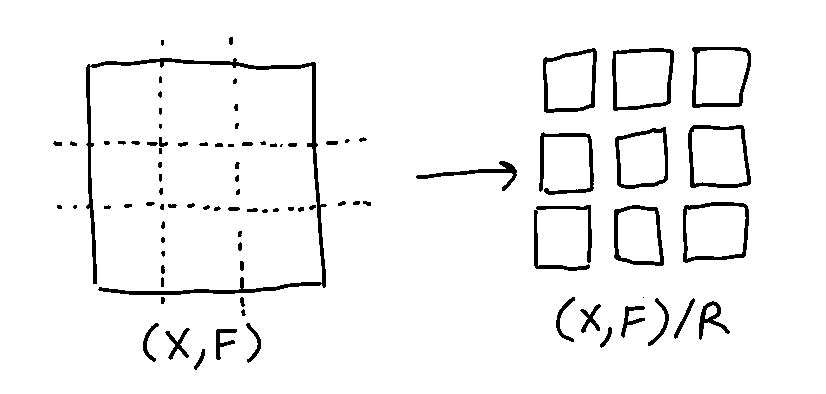
\includegraphics{/images/export-11.png}
\caption{An intuitive representation of a quotient algebra, where the dotted lines represent the congruence $R$ on the algebra $(X, F)$. }
\end{figure}

The fact that you can only form a quotient algebra over a congruence relation may remind you of the fact that \href{https://mathworld.wolfram.com/QuotientGroup.html}{you can only form a quotient group over a normal subgroup}. In fact, \textbf{congruences on groups are isomorphic to normal subgroups}: for any group $(X, \ast, i, ^{-1})$ and congruence $R$, the set of all $a$ in $X$ such that $R(a, 1)$ forms a normal subgroup of $(X, \ast, i, ^{-1})$. 

To see this, recall that a normal subgroup $N \subseteq X$ is defined by the fact that for all $b \in X$, $b N b^{-1} = \{b \ast n \ast b^{-1} | n \in N\} = N$. Let $H = \{a | R(a, 1)\}$. For any $b \in X$, reflexivity of $R$ implies that $R(b, b)$ and $R(b^{-1}, b^{-1})$. The fact that $R$ preserves operations implies that for any $a$ such that $R(a, 1)$, $R(bab^{-1}, b1b^{-1}) = R(bab^{-1}, 1)$, which in turn implies that $bHb^{-1} = H$, satisfying the definition of a normal group.

Conversely, if $N$ is a normal subgroup of $(X, \ast, i, ^{-1})$, then the relation $R$ where $R(a, b)$ if and only if $a \ast b^{-1}$ in $N$ is a congruence relation. Reflexivity holds because all normal subgroups must contain $b \ast b^{-1} = 1$. Symmetry holds because normal subgroups must be closed under inverse, and $(a \ast b^{-1})^{-1} = b \ast a ^{-1})$. Transitivity holds because all subgroups must be closed under $\ast$, and $( a \ast b^{-1}) \ast (b \ast c^{-1}) = a \ast c^-1.$ Preservation of operation holds because normal subgroups contain the identity, are closed under inverse, and are closed under multiplication.

Congruences on lattices lack an analogue as exciting as normal subgroups. R is a lattice congruence on $(X, \land, lor)$ if and only if for all $a, b, c, d \in X$, $R(a, b)$ and $R(c, d)$ imply that $R(a \land c, b \land d)$ and $R(a \lor c, b \lor d)$, which is just a straightforward application of the definition of a congruence.

\subsection{References}

Burris, S., & Sankappanavar, H. P. (2011). \textit{A Course in Universal Algebra (Graduate Texts in Mathematics, 78)} http://www.math.uwaterloo.ca/~snburris/htdocs/ualg.html

Dummit, D. S., & Foote, R. M. (2003). \textit{Abstract Algebra, 3rd Edition} (3rd ed).
\end{document} % This is the end of the document